\documentclass[10pt, twocolumn]{IEEEtran}
\usepackage{amsfonts, amsmath, amssymb, epsfig, graphicx}

\newcommand{\n}{\noindent}
\newcommand{\field}[1]{\mathbb{#1}}
\newcommand{\D}[2]{\frac{\partial #2}{\partial #1}}
\newtheorem{theorem}{Theorem}
\newtheorem{lemma}[theorem]{Lemma}
\newtheorem{corollary}[theorem]{Corollary}
\newtheorem{definition}{Definition}
\newcommand{\thmend}{\hspace*{\fill}~\QEDopen\par\endtrivlist\unskip}
\newcommand{\eqdef}{ \stackrel{\bigtriangleup}{=} }
\newcommand{\e}{\epsilon}
\oddsidemargin  0.0in \evensidemargin 0.0in \textwidth      6.25in
\headheight     0.0in \topmargin      0.0in \textheight 9.25in
%\allowdisplaybreaks[4]
 % peanut gallery comments
%
%
% NOTE: Comment *in* the line below if you want a draft with no red comments.
% NOTE: Doing so may replace some of the red comments with 
%       extra spaces or newlines.
%\def\noeditingmarks{}
%
\newcommand{\textred}[1]{\textcolor{red}{#1}}
\ifx\noeditingmarks\undefined
  \newcommand{\pgwrapper}[2]{\textred{#1: #2}}
\else
  \newcommand{\pgwrapper}[2]{}
\fi


\begin{document}

\title{Information Theory in Economics and Investment}
\author{Preston Hansen\\
{\it University of Illinois at Chicago} \\
E-mail: phanse4@uic.edu}
\maketitle

\begin{abstract}
\end{abstract}

\section{Introduction}

Big results in information theory applied to economics and investing. Hopefully a look at open problems.

\section{Information Theory in Economics}

\subsection{Rational Inattention - Modeling behavior in the absence of perfect information}
Discuss rational inattention (especially in the context of typical models of behavior in economics).

Also discuss results and newer papers.
\subsection{Robustness}
Similar motivation to rational inattention.

Again discuss results and newer papers.
\subsection{Credit Risk Modeling}
Info theory used to develop AIC - used in all sorts of model validation.

One paper also uses AIC to look at the predictability of the stock market historically.
\section{Information Theory in Investment}
Some of the results below deal with the value or influence of information on invenstment in a
somewhat less information-theoretic centered approach (though in the abstract they still present
a quantification of information, and so they are worth considering/contrasting with the other
results).
\subsection{Value of Information}

\subsection{Value of Information in Biology}
The results above are extended and used to model a population as a financial portfolio in \cite{Rivoire2011}.
The growth rate of a population is, using virtually the same setup, bounded by the mutual information between
a set of variables representing the environment, and some signal in the environment,  $I(X_{t};Y_{t})$.
Notably, this bound is shown to not hold when considering that in contrast to financial models, biological populations
must process information at an individual level. This leads to the result that
\begin{gather*}
  I(X_{t};Y_{t}) \le I_{p}^{q_{env},q_{in}} \le I(X_{t};X'_{t})
\end{gather*}
i.e. in general the information gathered by any member of a population is less than the collective information
gathered by the entire population.
\subsection{Universal Portfolios}
Consider a stock market vector given by
\begin{gather*}
  \boldsymbol{x} = (x_{1}, x_{2}, ..., x_{m})^{t}
\end{gather*}
where $x_{i}$ is the price relative of a given stock - the ratio of its closing to opening price - for a given day.

A portfolio is defined as
\begin{gather*}
  \boldsymbol{b} = (b_{1}, b_{2}, ..., b_{m})^{t}, b_{i} \ge 0, \Sigma b_{i} = 1.
\end{gather*}
where each $b_{i}$ represents the proportion of current wealth invested in stock $i$.

Finally, the factor by which wealth increases
in a given investment period, $S$, can then be defined as $ S = \Sigma b_{i}x_{i} $
A straightforward comparison can be made between any two investment strategies by comparing $S$ for various scenarios.

In \cite{universal}, a strategy is shown that achieves $S_{n}$ ($S$ over a sequence of n stock vectors) equal to,%
in the first order of the exponent, the best constant rebalanced portfolio $S^{*}_{n}$. 



\subsection{Influence of Side Information in Investment}
additional result from optimal portfolios above
\subsection{Cost of Achieving the Best Portfolio in Hindsight}


%You can include figures such as \ref{fig:owl}  in .eps, .jpg, .pdf format like this:

% \begin{figure}[h]
% 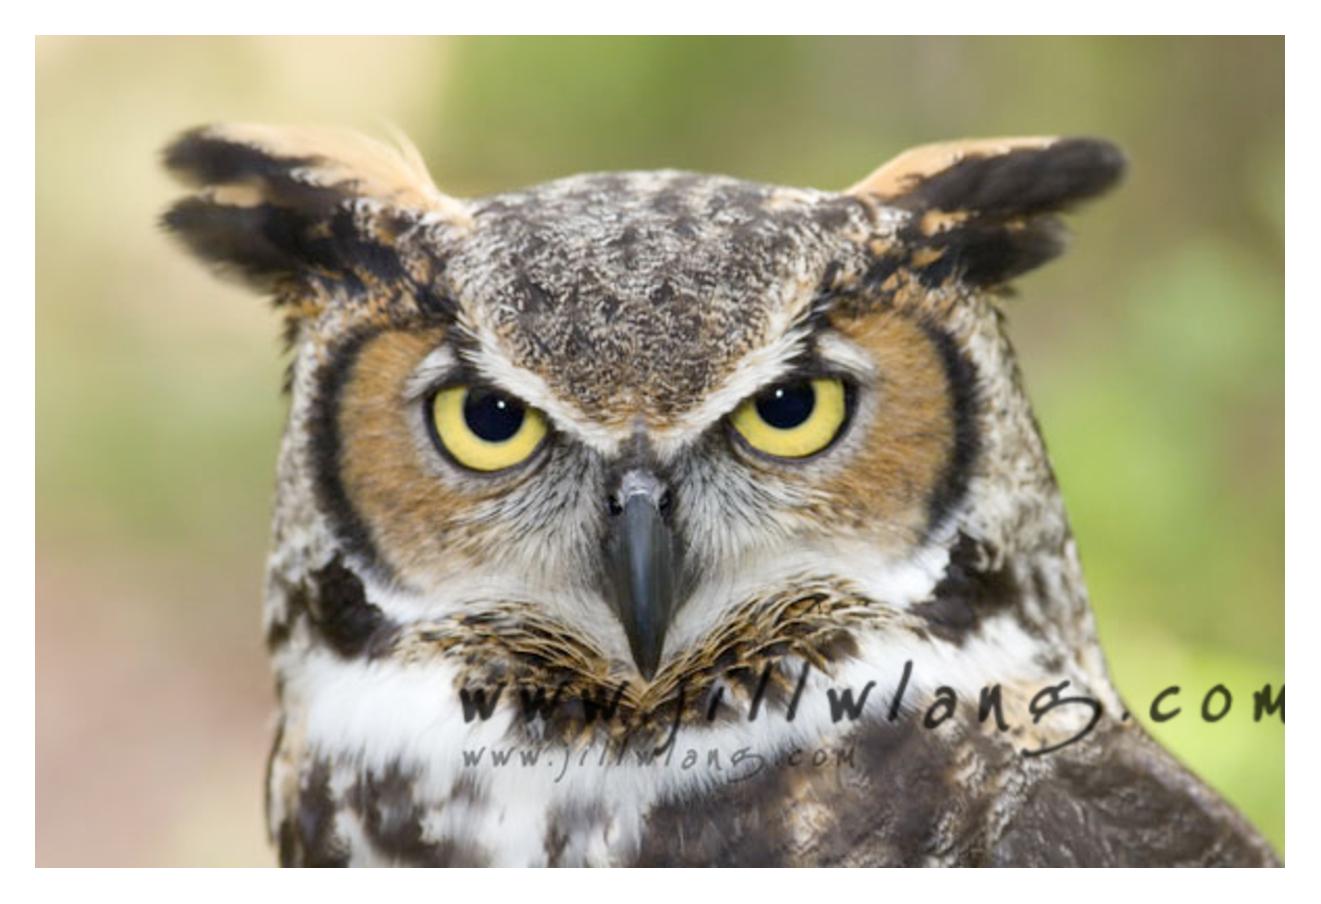
\includegraphics[width=8cm]{owl}
% \centering \caption{Great horned owls are great.}
%  \label{fig:owl}
% \end{figure}

%I can reference files in the {\tt refs.bib}.

running refs list: \cite{RePEc:eee:monchp:3-04}, \cite{Burnham2011}, \cite{Cover2005}, \cite{Cover1988},

\cite{Cover1998}, \cite{Li2017}, \cite{Sims2003}, \cite{Woodford2009}, \cite{Hansen2010}, \cite{StochasticGames},

\cite{Pesaran1995}


 
\baselineskip=2pt
\bibliographystyle{IEEEtrans}
\bibliography{refs}

\end{document}
